
\documentclass[a4paper,11pt,twoside]{scrartcl}
\usepackage[utf8x]{inputenc}
\usepackage{graphicx}
\usepackage{geometry}
\usepackage[ngerman]{babel}
%\usepackage{babelbib}
%\usepackage[backend=biber]{biblatex}
\usepackage{units}
\usepackage{url}
\usepackage{setspace}
\usepackage[
	pdftitle={Energie_Suffizienz},
 	pdfauthor={et.al.},
% 	pdfsubject={},
% 	pdfkeywords={},
	pdfstartview=FitH, % Auf Seitenbreite anpassen (Anzeige)
	pdfborder={0 0 0},
%  	bookmarks=true,
% %	plainpages=false,
	colorlinks=false,
	hyperfootnotes=false,
	pagebackref=false]{}
\usepackage[colorinlistoftodos,prependcaption,textsize=normalsize]{todonotes}  % disable
\usepackage{amsmath}
\usepackage{amstext}
\usepackage{amssymb}
\usepackage{color}
\usepackage[numbers]{natbib}
\usepackage{pdfpages}
\usepackage{hyphenat}
\usepackage{pdflscape} % für drucken ändern auf package lscape /pdflscape
\usepackage{textpos}
\usepackage{microtype}
\usepackage{enumitem}
\usepackage{multirow}
\usepackage{pdfcomment}

\usepackage{pgfgantt} % gantchart für den Arbeitsplan

% \usepackage{hyphenat}
\usepackage{float}
\usepackage{placeins}
\RequirePackage[bf]{caption}

\renewcommand{\textfraction}{.01} % vorher: .2
\renewcommand{\floatpagefraction}{.99}% vorher: .5
\renewcommand{\topfraction}{0.9}	% max fraction of floats at top
\renewcommand{\bottomfraction}{0.9}	% max fraction of floats at bottom

\newcommand{\ltab}{\raggedleft\arraybackslash}
\newcommand{\ctab}{\centering\arraybackslash} 
\newcommand{\rtab}{\raggedright\arraybackslash}

\usepackage{tabularx}
\newcolumntype{L}[1]{>{\raggedright\arraybackslash}p{#1}} % linksbündig mit Breitenangabe
\newcolumntype{C}[1]{>{\centering\arraybackslash}p{#1}} % zentriert mit Breitenangabe
\newcolumntype{R}[1]{>{\raggedleft\arraybackslash}p{#1}} % rechtsbündig mit Breitenangabe

\newcommand{\rem}[1]{}

% \renewcommand{\figurename}{Abb.}
% \renewcommand{\tablename}{Tab.}

\usepackage{acronym}
%\renewcommand{\bflabel}[1]{\normalfont{\normalsize{#1}}\hfill}

\usepackage[automark]{scrpage2}
\pagestyle{scrheadings}
\clearscrheadfoot
\ohead{\headmark}
\ofoot{\pagemark}
\setheadsepline{0.4pt}
\setfootsepline{0.4pt}

\setkomafont{pageheadfoot}{\rmfamily\small}

\renewcommand{\thefigure}{\arabic{section}-\arabic{figure}}
\renewcommand{\thetable}{\arabic{section}-\arabic{table}}

\newcommand{\entspricht}{\mathrel{\widehat{=}}}

\geometry{left=25mm,right=25mm, top=28mm, bottom=28mm}
\parindent 0pt
\parskip 11pt

% kein Platz zwischen \items
\setlist{nosep}
% Platz nach Überschriften reduzieren
\usepackage{titlesec}
\titlespacing*{\section}{0pt}{0pt}{0pt}
\titlespacing*{\subsection}{0pt}{0pt}{0pt}
\titlespacing*{\subsubsection}{0pt}{0pt}{0pt}
\titlespacing*{\paragraph}{0pt}{0pt}{5pt} % horizontal spacing in paragraph

\begin{document}
\onehalfspacing

\clearpage


{\singlespacing

\thispagestyle{empty}
\begin{center}

%first row logos
\begin{figure}[htb]
    \centering
    \begin{minipage}[c]{0.3\linewidth}
        \centering
        
\includegraphics[width=4.5cm]{logos/europa-universitaet-flensburg-hauptlogo-rgb-600dpi.png}
    \end{minipage}
    \hfill
    \begin{minipage}[c]{0.35\linewidth}
        \centering
        \includegraphics[width=5cm]{logos/Logo_interdiszi_institut.png}
    \end{minipage}
    \hfill
    \begin{minipage}[c]{0.3\linewidth}
        \centering
        \includegraphics[width=2.5cm]{logos/Logo_wuppertal.png}
    \end{minipage}
\end{figure}

\iffalse
%second row logos
\begin{figure}[htb]
    \centering
    \begin{minipage}[c]{0.3\linewidth}
        \centering
        \includegraphics[width=2.2cm]{logos/2015_Logo_TUM_RGB.jpg}
    \end{minipage}
    \hfill
    \begin{minipage}[c]{0.35\linewidth}
        \centering
        \includegraphics[width=5.5cm]{logos/isea_rwth_logo.jpg}
    \end{minipage}
    \hfill
    \begin{minipage}[c]{0.3\linewidth}
        \centering
        \includegraphics[width=3cm]{logos/TU_Logo_lang_RGB_rot.png}
    \end{minipage}
\end{figure}
\fi
\vspace*{1 cm}

{\LARGE\textbf{\textsf{Skizze Nachwuchsforschungsgruppe}}

\textsf{\textit{im Rahmen der Bekanntmachung \glqq inter- und transdisziplinär arbeitende Nachwuchsgruppen im Rahmen der Sozial-ökologischen Forschung\grqq} }
}

\vspace{0.5cm}

{\Huge
\textbf{\textsf{Die Rolle von Energie-Suffizienz in Energiewende und Gesellschaft}}

\textbf{\textsf{}}
}

{\Huge
\textbf{\textsf{Akronym:{EnSufGe}}}
}

\vspace{1cm}

Eingereicht durch
Frauke Wiese\\
i$^{2}$ Interdisziplinäres Institut für Umwelt-, Human- und Sozialwissenschaften\\
Europa-Universität Flensburg, Auf dem Campus 1, 24943 Flensburg


\vspace{0.5cm}

An den Projektträger im DLR \\
AE 41 Globaler Wandel/Klima- und Umweltschutz, Sozial-ökologische Forschung \\
Heinrich-Konen-Straße 1, 53227 Bonn


\end{center}
\iffalse
\begin{table*}[b]
\centering
\footnotesize
\begin{tabular}{ | p{5cm} | p{5cm} |} \hline
\textbf{Konsortialpartner} & \textbf{Modelle/Frameworks} \\ \hline
Reiner Lemoine Institut & Leitung des Experiments \\ \hline
Technische Universität München & urbs \\ \hline
Europa-Universität Flensburg & oemof \\ \hline
RWTH Aachen & GENESYS-2 \\ \hline
Technische Universität Berlin & OSeMOSYS \\ \hline
Dänische Technische Universität & Balmorel \\ \hline
\end{tabular}
\label{tab:Partner}
\end{table*}
\fi


\clearpage
}

\setcounter{page}{1}

\section{Zielstellung und gesellschaftlicher Bedarf}
\label{sec:ziel}
%\textit{Beschreibung der Problem- und Zielstellung sowie des gesellschaftlichen Bedarfs}

Klimawandel, Ressourcenverknappung und zunehmende Umweltveränderungen lassen die Transformation des Energiesystems zu einer der zentralen gesellschaftlichen Herausforderungen werden. Noch ist weitgehend offen, wie die Versorgung mit Strom, Wärme, Mobilität sichergestellt werden kann, während Klimaziele erreicht, soziale Gerechtigkeit gewahrt und die natürlichen Grenzen unseres Planeten langfristig eingehalten werden können. 

Energiesystem-Modelle haben sich als Werkzeuge etabliert, um technisch mögliche und ökonomisch vorteilhafte Energiewende-Pfade darzustellen und zu analysieren. Sie helfen dabei, komplexe Zusammenhänge zwischen technischen Möglichkeiten (z.B. Flexibilität), Umweltbedingungen (z.B. Wetter-abhängige Erneuerbare), Marktregeln (z.B. Energy-only-Markt) im Licht klimapolitischer Zielsetzungen zu verstehen und unterstützen somit die Klima- und Energiepolitik.

Ein entscheidender Einflussparameter für berechnete Szenarien ist die zukünftige Nachfrage nach Strom, Wärme und Mobilität. Die Mehrzahl der bisherigen Modelle legt den Fokus  auf die Bereitstellung von Energiedienstleistungen. Die Nachfrage-Seite wird meist nur innerhalb enger Grenzen variiert. So berücksichtigen viele Modelle beispielsweise die Verschiebung der Nachfrage von fossilen Brennstoffen zu Strom durch die Elektifizierung im Wärme- und Transportsektor. Eine übergreifende Perspektive, welche die verschiedenen Bereiche berücksichtigt und integriert, in denen Energie gebraucht wird, steht noch aus. Zudem wird in den meisten Modellen die absolute Nachfrage nach Energie nicht in Frage gestellt. Mit anderen Worten: Bislang sind Modellierungen weitgehend blind gegenüber Veränderungen der Nachfrage nach Energie durch gesellschaftlichen Wandel oder Verhaltensänderungen.

Nicht nur in der Modellierung von Energiewende-Pfaden, sondern auch  bei Klimaschutz-Strategien liegt der Fokus bisher auf im weitesten Sinn technikorientierten Lösungen bei der Erzeugung und Distribution von Energie für Wohnen, Bauen, Ernährung und Mobilität \cite{Creutzig2018}. 

Zwar bieten laut Modellrechnungen Erneuerbare Energien und Effizienz die Möglichkeit im Jahr 2050 80-95 Prozent Treibhausgas-Reduktion in Deutschland \cite{BMWi2017} zu erreichen. Es gibt jedoch verschiedene Gründe keine der drei Nachhaltigkeitsstrategien Konsistenz (Erneuerbare Energien ersetzen Fossile), Effizienz (relative Reduktion des Energieverbrauchs bei Bereitstellung der gleichen Energiedienstleistung) und Suffizienz (absolute Reduktion der Nachfrage nach Energiedienstleistungen durch veränderte soziale Praktiken und gesellschaftliche Leitbilder) außer Acht zu lassen: Zum einen setzten die ambitionierten Ziele des Pariser Klimaabkommens die Herausforderung nochmal auf eine neue Stufe \cite{Rogelj2018}. Außerdem sprechen Aspekte wie Flächenverbrauch (Referenz fehlt noch), Ressourcenbedarf (Referenz fehlt noch) und Akzeptanzfragen \cite{Fuchs2016}, zusammengefasst die Einhaltung der planetaren Grenzen \cite{Rockstroem2009} dafür, die Chancen, die Suffizienz bietet, nicht zu übersehen \cite{SAMADI2017}.

Desweiteren ist bisher nicht abschließend geklärt, in welchem Ausmaß Emissionsreduktionen in Deutschland durch Konsistenz und Effizienz tatsächlich erreicht wurden. Verlagerungseffekte in andere Länder könnten ebenso eine Rolle gespielt haben \cite{Wiedmann2015}, so dass die Emissionsreduktionen bei Bilanzierung nach Verursacherprinzip geringer ausfallen würden. Auch die Rolle, die Effizienz spielen kann, ist nicht klar. Zielszenarien für Deutschland gehen von einer Reduzierung der Stromnachfrage durch eine massive Steigerung von Effizienz aus \cite{BMWi2017}. Zugleich findet jedoch in der fachwissenschaftlichen und energiepolitischen Diskussion der Befund Aufmerksamkeit, dass Energieeffizienzsteigerungen in der Regel von Rebound-Effekten begleitet werden, welche die Einsparungen teilweise kompensieren oder mitunter sogar zu einem verstärkten Energieverbrauch („Backfire“) führen \cite{DeutscherBundestag2013,Santarius2012}. Auch aufgrund solcher Rebound-Effekte wurden in den vergangenen Jahren die Energiesparpotenziale nicht voll ausgeschöpft, was dazu beitrug, dass in Deutschland trotz aller Maßnahmen zur Verbesserung der Energieeffizienz der Stromverbrauch im Jahr 2016 gegenüber 2008 (acht Jahre) um nur 1,5 Prozent gesunken ist \cite{UBA2017}. Dies lässt das erklärte Ziel weitere 8,5 Prozent bis 2020 (vier Jahre) zu schaffen sehr ambitioniert erscheinen.

In Anbetracht des möglichen Beitrags der Suffizienz und der Größe der Herausforderung, ist die Rolle von Energie-Suffizienz derzeit unterrepräsentiert in Diskussion und Forschung für Klimaschutz und Energiewende. Abbildung \ref{fig:zusammenspiel} verdeutlicht schematisch den Gedanken des Zusammenspiels der drei Dimensionen für die Erreichung der Klimaziele. 


\begin{figure}[!h]
    \centering
    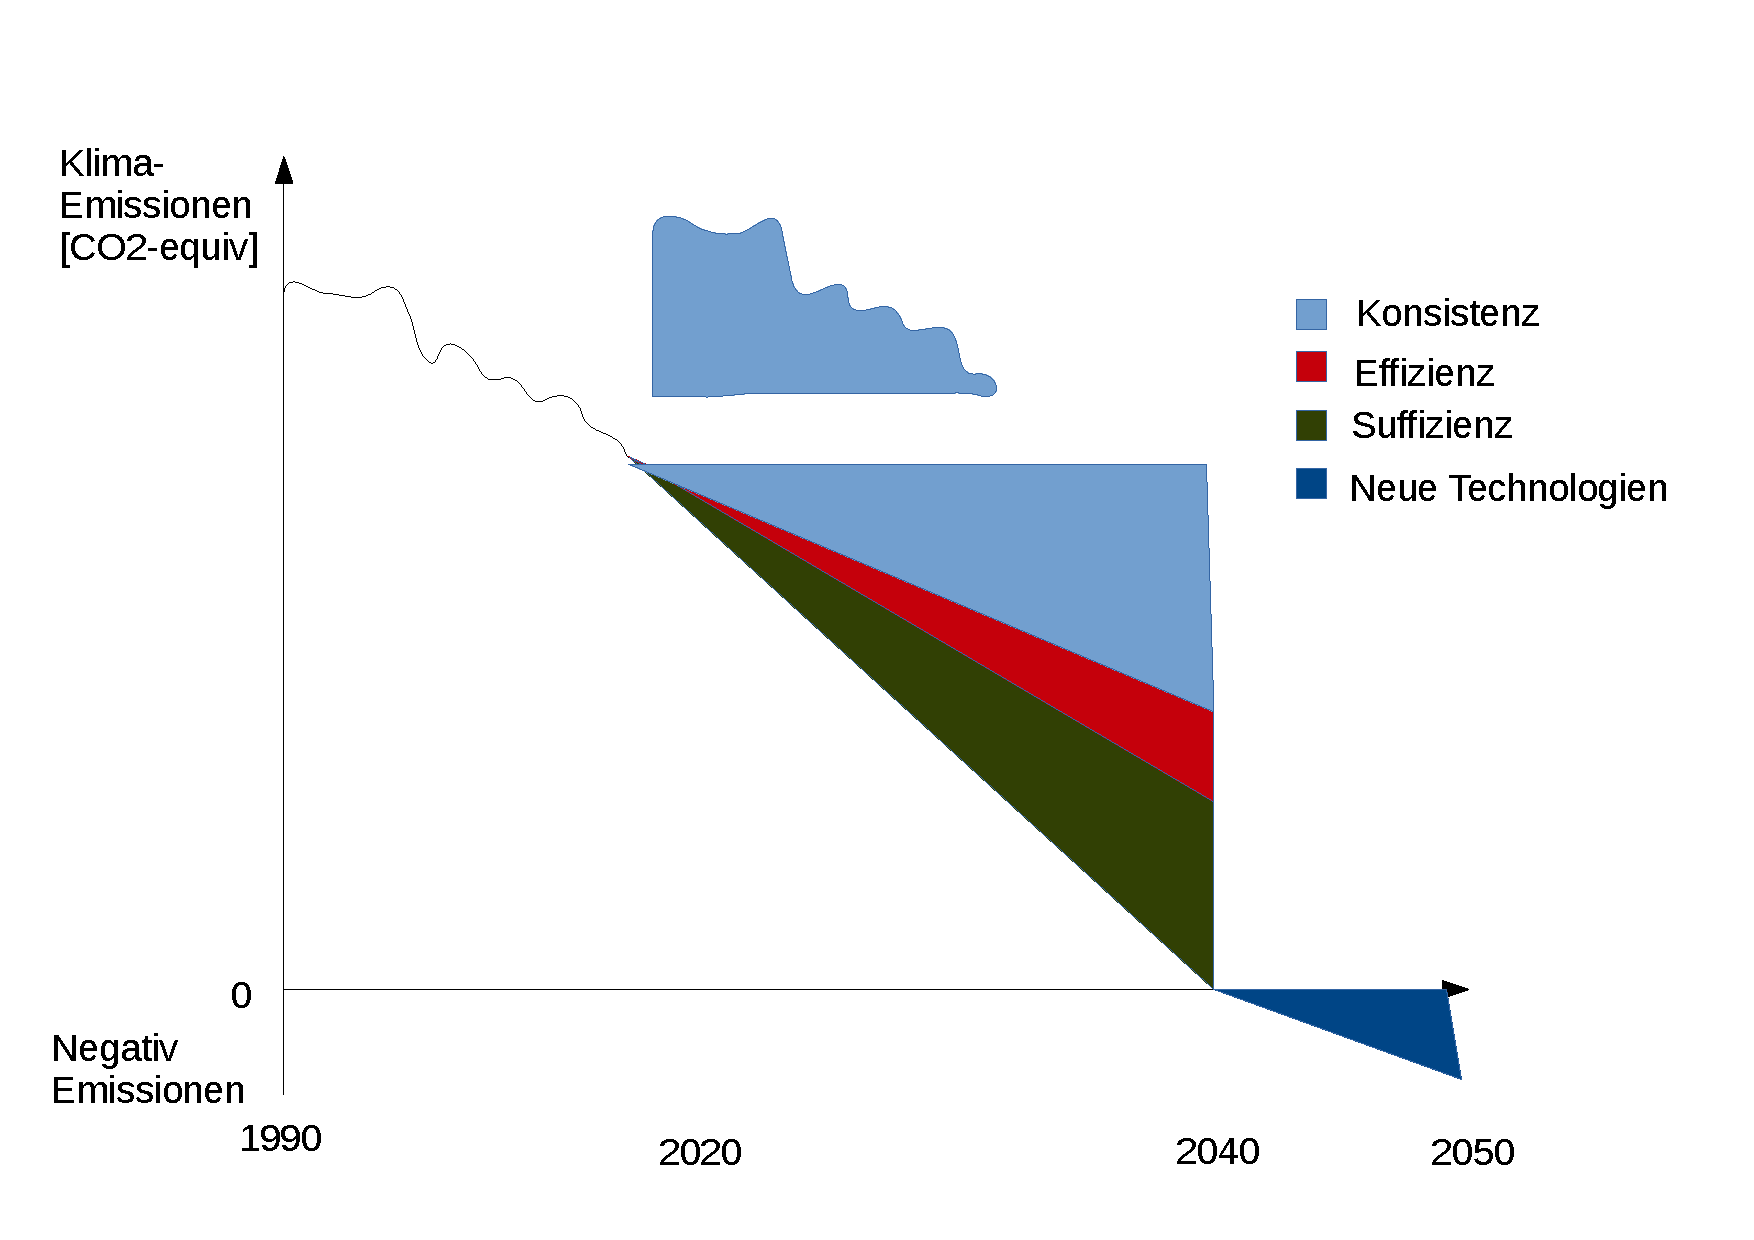
\includegraphics[width=0.8\textwidth]{figures/Zusammenspiel2.pdf}
    \caption{Schamatisch: Bisherige Emissionsreduktion durch Konsistenz (links), notwendiger Beitrag von Effizienz und Suffizienz in Zukunft (rechts) zur Erreichung der Klimaziele in Deutschland}
    \label{fig:zusammenspiel}
\end{figure}

Weiter hat sich in der Forschung die Erkenntnis durchgesetzt, dass sich nur unter Einbeziehung und dem Zusammenspiel verschiedener Disziplinen - wie technisch-/ingenieurwissenschaftlicher Fachrichtungen, Politik-, Wirtschafts- und Sozialwissenschaften - die gesellschaftliche Herausforderung der Transformation des Energiesystems erfolgreich bewältigen lässt \cite{WGBU2012}.

Besonders deutlich wird die Notwendigkeit der verstärkten interdisziplinären Zusammenarbeit bei der Erstellung von Energie-Szenarien. Gesellschaftliche Entwicklungen haben enormen Einfluss auf die Nachfrage nach Energie-Dienstleistungen, die politischen Rahmenbedingungen für die Erzeugungs- und Distributionswege sowie die technisch-ökonomischen Optionen zur Erfüllung der Energienachfrage (schematisch dargestellt in Abbildung \ref{fig:szenarien}). Gängige Praxis in der Energiesystem-Modellierung ist es, nur Letzteres in den Blick zu nehmen, gesellschaftliche Dynamiken hingegen weitgehend zu ignorieren (Abbildung \ref{fig:szenarien} links). Dieses Vorgehen erlaubt eine Abschätzung der Leistungsfähigkeit sozio-technischer Innovationen. Allerdings um den Preis einer Vorstellung, die Gesellschaft als mehr oder weniger statisches Konstrukt imaginiert und nicht als das hoch dynamische, beständigen Veränderungen unterworfene Gemeinwesen, das sie ist. Für konsistente und damit belastbare Energie-Szenarien ist die Integration sozialwissenschaftlicher Wissensbestände in Bezug auf künftig zu erwartende gesellschaftliche Transformationsprozesse und ihre Auswirkungen auf den gesellschaftlichen Metabolismus unverzichtbar. Beispielhaft seien hier die Digitalisierung oder der demografische Wandel genannt. Beide Prozesse werden mit hoher Wahrscheinlichkeit Auswirkungen auf die Nachfrage nach Energiedienstleitungen haben, in welchem Umfang und in welche Richtung - steigende oder sinkende Nachfrage - ist erstens kontingent und zweitens allein mit Verweis auf die Leistungsfähigkeit technischer Innovationen nicht zu beantworten. Noch nicht abzusehen ist auch, in welchem Ausmaß etwa kommunale und nationale Klimaschutzmaßnahmen - erinnert sei hier an die aktuelle Diskussion um den ticketlosen ÖPNV - soziale Innovationen oder einen Wandel gesellschaftlicher Werte und Normen beeinflussen werden. Außerdem ermöglicht die Erweiterung des Bezugsrahmens um die gesellschaftliche Perspektive (Abbildung \ref{fig:szenarien} rechts), Suffizienz neben Effizienz und Konsistenz in der Modellierung abzubilden. 

\begin{figure}[!h]
    \centering
    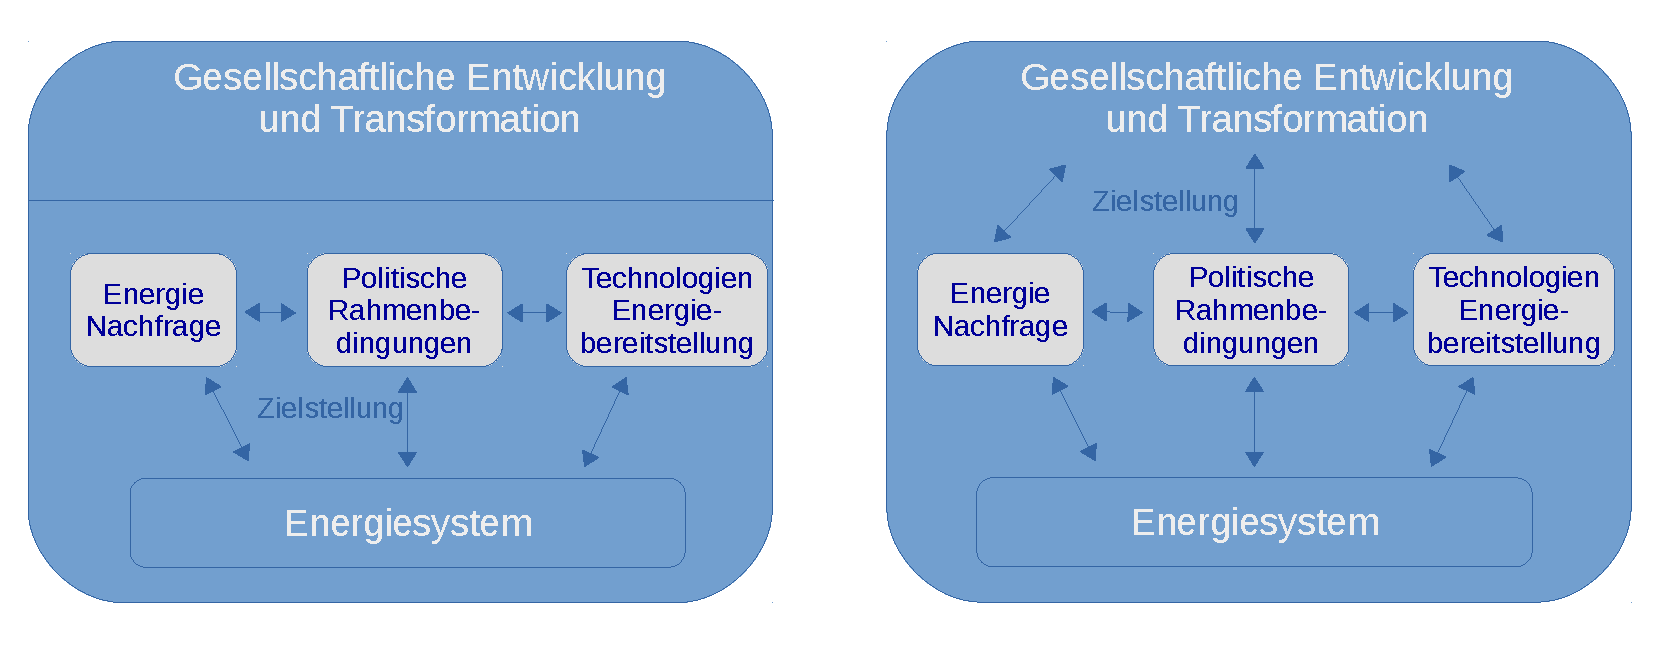
\includegraphics[width=0.8\textwidth]{figures/Szenarien.pdf}
    \caption{Rahmen für Energie-Szenarien: Links: Getrennte Betrachtung / Rechts: Einbettung der Annahmen für Energie-Nachfrage, Politikrahmen und technische Optionen in gesellschaftliche Entwicklungen}
    \label{fig:szenarien}
\end{figure}

Ziele der Nachwuchsforschungs-Gruppe Energie-Suffizienz sind:
\begin{itemize}
 \item Einen in der bisherigen Diskussion um die Transformation des Energiesystems in Richtung Nachhaltigkeit unterrepräsentierten Aspekt  -- Suffizienz -- intensiv dahingehend zu erforschen
  \item In der interdisziplinäre Kooperation ein Verfahren für die Erstellung von konsistenten, multiperspektivischen  Energieszenarien zu entwickeln und zu erproben
  \item (Weiter)-Entwicklung eines Energiesystem-Modells, in dem Konsistenz, Effizienz und Suffizienz integriert betrachtet werden können
 \item Einen möglichen und eventuell notwendigen Beitrag von Energie-Suffizienz zur Erreichung der Klimaziele auf nationaler (Deutschland) und kommunaler (Flensburg) Ebene ermitteln
 \item Die Entwicklung von Zukunftsszenarien zur Transformation des Energiesystems in Richtung Nachhaltigkeit 
 \item Die historische Rekonstruktion der Wechselwirkung zwischen Energiesystemtransformation und gesellschaftlichem Wandel  
 \item Handlungsoptionen für Suffizienz-Politik von kommunaler bis EU-Ebene
 \item Literatur und Methoden der Energiesystem-Analyse als auch die der sozial-ökologischen Transformationsforschung erweitern. Schwerpunkt liegt dabei auf Synergien zwischen den Forschungsgebieten.
 \item Das Methodenspektrum junger Forscher mit Hintergründen aus Sozialwissenschaft (sozial-ökologische Transformationsforschung), Wirtschaftingenieurwesen (Energiesystem-Analyse) und Politikwissenschaft interdisziplinär erweitern
\end{itemize}

Im Rahmen des Projektes erarbeitete Daten und Software, werden open source zur Verfügung gestellt. Der Open Science Ansatz, der der Nachwuchs-Forschungsgruppe zugrunde liegen wird, beinhaltet auch den offenen Zugang zu Publikationen etc. Die Erkenntnisse sollen außerdem politische Entscheidungsprozesse zu Klimaschutz und Energiewende unterstützen und Empfehlungen für Suffizienzpolitik beinhalten. Ein Schwerpunkt wird die Ergebnis-Kommunikation auch im populär-wissenschaftlichen Bereich, um auch eine außerwissenschaftliche Öffentlichkeit zu erreichen.

\section{Stand von Wissenschaft und Technik sowie eigene Vorarbeiten}
% gemeinsamer Anfang: UTAS input
%Hier zunächst ein den Verbund umfassender Vorspann, damit uns die Geschichte hier nicht sogleich in die verschiedenen Verbundpartner*innen zerfällt. Ich erzähle von hinten nach vorn (erst Suffizienz, dann Transformation und dann Energiesystem-Analyse und Modellierung, damit es dann zu Fraukes Part überleitet).
Nachhaltigkeitsforschung, sozial-ökologische Forschung und Transformationsforschung sind seit langem mit Fragen der „Umsetzung“ befasst: Wie ist es möglich, vom Wissen zum Handeln zu kommen (ältere BMBF-Ausschreibung der SÖF hieß so); wie kann geschehen, was geschehen muss (###gleichnamige Festschrift für Manfred Linz zum 75. Geburtstag) und wie können Klimaschutzziele, wie kann ein deutlich geringerer Naturverbrauch erreicht werden, ohne zivilisatorische Errungenschaften zu gefährden (###WBGU-Gutachten zur Großen Transformation und ###Bernd Sommer und Harald Welzer  2014)? Die Antworten fallen unterschiedlich aus und die Bearbeitung dieser Frage geschieht in unterschiedlicher Weise. So hat der Nachhaltigkeitspfad der Suffizienz lange im Schatten von Effizienz (mehr Wohlstand bei geringerem Ressourcenverbrauch) und von Konsistenz (Wechsel der Stoffbasis) gestanden (###Winterfeld). Die Transformationsforschung hat sich zunächst stark am von der System- und Managementtheorie kommenden Transition-Ansatz orientiert (### Rotmans, ###Geels 2004; ### Loorbach 2010). Innerhalb der Debatten haben Szenarien und Modelle zum einen stets die Funktion gehabt, Orientierungswissen zu generieren zu zeigen, dass beispielsweise eine Energiewende (Ausstieg aus der Atomenergie und Umstieg auf erneuerbare Energieträger) möglich ist. Zugleich sind sie allerdings wegen ihrer Lebensweltferne und wegen ihres Abstraktionsgrades immer auch kritisiert worden. Wolfgang Sachs hat für das Wuppertal Institut die Fraktion der „Zähler“ von der Fraktion der „Erzähler“ unterschieden und in der ersten Studie „Zukunftsfähiges Deutschland“ ist versucht worden, beide Ebenen zu bedienen und versuchsweise zu vermitteln (### BUND; Misereor 1996).

\subsection*{Energiesystem-Analyse und Modellierung}
% ESM wichtig in Politik-Beratung
Trotz existierender Kritik, nehmen Energiesystem-Modelle eine wichtige Rolle in Wissenschaft und politischer Beratung zu Klima- und Energiepolitik ein \cite{Dieckhoff2015}.

% Entwicklung
Wurde Energiesystem-Modellierung in ihrer Anfangszeit in den 1950ern nur zur Planung neuer Kapazitäten genutzt \cite{Kagiannas2004}, nahm die Bedeutung für die Planung von nachhaltigeren Energiequellen nach der Ölkrise in den Siebzigern zu \cite{Wei2006}. Ein wichtiger Beitrag der Modelle war es dann, die Realisierbarkeit von 100\% Erneuerbare Energien Strom-Systemen darzulegen, sowohl für Deutschland \cite{SRU2011} als auch für Europa \cite{Hohmeyer2015}. Inzwischen geht es nicht mehr um das ob, sondern eher um das wie der Energiewende. Modelle tragen u.a. zu Fragen der Marktregeln, optimalem Mix von Wind und Solar, Netz- und Speicherbedarf bei.  

% Komplexität erhöht sich
Da die Bedeutung der Sektorkopplung zunimmt \cite{Quaschning2016} hat sich die integrierte Betrachtung der Sektoren Strom, Wärme, Mobilität inzwischen etabliert. Gleichzeitig nimmt die zeitliche und räumliche Auflösung der Modelle zu, um Effekte von fluktuierender Einspeisung von Wind und Solar besser abbilden zu können. Genauso wie die Anzahl hat auch die Komplexität der Modelle in den letzten Jahren stark zugenommen.

% Transparenz wichtig für Partizipation wichtig
In den letzten Jahren wurden die Modelle verstärkt für ihren Black-Box-Charakter kritisiert \cite{Pfenninger2017, Pfenninger2017b,Cao2016}. \cite{Wiese2015} formuliert den Bedarf an Transparenz in der Energiesystem-Modellierung um Partizipation zu ermöglichen \cite{Wiese2014} als Grundlage für Transparenz, die essentiell für eine partizipative Energiewende ist.

% Interdisziplinär wichtig, Sozialwissenschaft unterrepräsentiert
Außerdem wird zunehmend ein Bedarf an interdisziplinären Ansätzen in der Energiesystem-Modellierung identifiziert \cite{Wiese2018,Pfenninger2014,Schuitema2017}. Die Sozialwissenschaft ist unterrepräsentiert in Energieforschung \cite{Sovacool2014}, was in Anbetracht der Relevanz der Sozialwissenschaften für eine gesellschaftliche Energiewende \cite{Sovacool2015} verwunderlich ist.

% Sozialwissenschaftliche Ansätze bisher
Ein Bereich, in dem sozialwissenschatliche Ansätze in der Energiewende-Modellierung bereits zur Anwendung kommen, ist die Forschung zu Akzeptanz von neuen Netzleitungen und Windkraftanlagen \cite{vernetzen2016} und dem Ausstieg aus der Kohlekraftwerken \cite{Heinrichs2017}.

% Gesellschaftliche Einbettung Szenarien
Um Modell-basierte Szenarien in einen gesellschaftlichen Kontext einzubetten, wenden \cite{WEIMERJEHLE2016} Kontext-Szenarien \cite{WEIMERJEHLE2006} an. Es gibt also erste Ansätze in  sozio-technischen Energieszenarien qualitative und quantitative Elemente der Systemanalyse zu verknüpfen.

% Suffizienz in der Energiesystem-Modellierung quantifiziert?
Trotzdem gibt es noch wenige Energieszenarien, die Suffizienz in die Analyse aufnehmen. Eine Ausnahme ist das französische Negawatt-Szenario, das Suffizienz neben Konsistenz und Effizienz abbildet \cite{negawatt2017} und mit halbiertem Energieverbrauch bei bleibendem hohen Standard an Energiedienstleistungen kalkuliert. Eine Analyse verschiedener Energie-Szenarien zeigt jedoch, dass Suffizienz trotz des potentiellen Beitrags kaum untersucht wird \cite{SAMADI2017}.

% WEITERE NOTIZEN
% Wichtig andere Aspekte miteinzubringen, Perspektive der Resilienz als verknüpfendes Element \cite{Wiese2016}.
% Es gibt immer implizite Annahmen in Energieszenarien
% (Johannes): Energieszenarien für DE (HERON-Projekt, LEAP)

\subsection*{Sozial-ökologische Transformationsforschung}
\textit In der interdisziplinären Nachhaltigkeitsforschung ist in den vergangenen Jahren ein neuer Forschungszweig entstanden, der sich mit der gesellschaftlichen Transformation in Richtung Nachhaltigkeit befasst. Gesellschaftliche Transformationsprozesse werden hier als zukunfts-orientierte Gestaltungsaufgabe verstanden (Sommer und Welzer 2014). Dies gilt auch für die Transformation des Energieregimes. Dass die Etablierung einer klimafreundlichen und nach-haltigen Energieversorgung grundsätzlich technisch machbar und ökonomisch zu bewältigen wäre, gilt als sehr wahrscheinlich. Dafür, dass dies trotz der Virulenz der Klimakrise nicht (bzw. nicht in der gebotenen Geschwindigkeit) geschieht, werden vor allem gesellschaftliche Barrieren und Zwänge ausgemacht. Im Zentrum des Interesses stehen daher gesellschaftli-che Fragen einer solchen Nachhaltigkeitstransformation, wie Governance-Aspekte sowie nachhaltige soziale Praktiken und die Bedingungen ihrer Diffusion.
Die Geschichte der Energieproduktion und der Energienutzung ist eine der permanenten Effizienzsteigerungen und zugleich eine des sukzessiven Verlustes nachhaltiger, damit auch suffizienter gesellschaftlicher Reproduktion und entsprechender sozialer Praktiken. Histo-risch betrachtet lässt sich konstatieren: Die energetische Dichte der verwendeten Rohstoffe nahm in den vergangen rund 300 Jahren mit jeder neuen Ressource zu (von Biomasse über Kohle zu Erdöl/Erdgas und atomare Energie). Zusätzlich ließen technische Innovationen die Ressourcenproduktivität steigen. Beides trug, vermittelt über sich verändernde soziale Ord-nungen, Lebensweisen und damit einhergehenden Normen- und Wertewandel, zu einer Steigerung des absoluten Ressourcen- und Naturverbrauchs bei (Krausmann und Fischer-Kowalski 2010). Heute sind diese Verbräuche auf einem historisch einzigartig hohen Niveau – mit gravierenden, zum Teil irreversiblen Folgen für Gesellschaften und Natur.
Vor dem Hintergrund der sozial-ökologischen Auswirkungen dieses hohen Naturverbrauchs, der Zerstörung von Ökosystemen, der zunehmenden Übernutzung ökologischer Senken sowie den unkalkulierbaren sozialen und ökologischen Risiken, die mit der Nutzung atomarer Energie verbunden sind, ist in Deutschland die Energiewende auf den Weg gebracht wor-den; vorbereitet, befördert und ermöglicht durch Jahrzehnte der umweltpolitischen und zivil-gesellschaftlichen Auseinandersetzungen einerseits und die Arbeit von Pionier*innen der regenerativen Energieversorgung andererseits (David und Schönborn 2016). Bei der Umset-zung der Energiewende kommen bisher vor allem technische Maßnahmen zum Einsatz. „Die Energiewende basiert auf zwei Säulen: erneuerbare Energien und Energieeffizienz“, heißt es entsprechend im Ersten Fortschrittsbericht zur Energiewende des Bundesministeriums für Wirtschaft und Energie (BMWi 2014: 5). Energiesuffizienz hingegen, das heißt die Begren-zung und langfristige Reduktion des absoluten Energieverbrauchs durch soziale Innovatio-nen, Exnovationen und verändertes Nutzungsverhalten, spielt bislang noch eine untergeord-nete Rolle – obwohl die Reflektion der bis dato ergriffenen Maßnahmen zeigt, dass diese zur Senkung des absoluten Verbrauchs nicht ausreichen werden (Brischke et al. 2016). Ohne Suffizienz wird die Energiewende, das wird in der sozial-ökologischen Forschung seit länge-rer Zeit thematisiert, nicht zu schaffen sein (Huber 1995; Fischer und Grießhammer 2013; Schneidewind und Zahrnt 2013). Um zu verstehen, wie Suffizienz, suffiziente Lebensweisen und soziale Praktiken eine breitere gesellschaftliche Basis erreichen kann, scheint ein Blick in die Vergangenheit als auch in die Zukunft sinnvoll und notwendig (siehe AP 2).
Das Norbert Elias Center for Transformation Design & Research (NEC) der EUF ist ein sozi-alwissenschaftliches Forschungszentrum zur Untersuchung gesellschaftlicher Verände-rungsprozesse, insbesondere in Hinblick auf Fragen der Nachhaltigkeit und Zukunftsfähigkeit zeitgenössischer Gesellschaften. Am Center werden historische Prozesse umfassenden gesellschaftlichen Wandels rekonstruiert, um aus den gewonnenen Erkenntnissen Hand-lungsoptionen, mögliche Entwicklungslinien und Gestaltungsszenarien für zeitgenössische und künftige sozial-ökologische Wandlungsprozesse abzuleiten (Christ 2015, 2016), als auch gegenwartsorientierte Fragestellungen zum Zusammenhang von Klima, Kultur und Nachhal-tigkeit bearbeitet (Sommer 2011; Sommer und Schad 2014; Stumpf et al. 2015; Sommer 2016).
Als Strategie die auf veränderte Handlungsmuster und Nutzungsaspekte zielt, steht Suffizi-enz im Fokus des BMBF geförderten Forschungsprojekts „Entwicklungschancen und -hemmnisse einer suffizienzorientierten Stadtentwicklung (EHSS)“ (2017-2020). In diesem Forschungsprojekt werden in vergleichender Perspektive und im Rahmen eines Reallabors auf kommunaler Ebene Erfolgsbedingungen und Barrieren suffizienzorientierter Stadtent-wicklung untersucht. Eine Suffizienzpolitik in der Stadtentwicklung schafft Strukturen, die suffizienzorientierte (Alltags-) Praktiken erleichtern – etwa im Bereich der Mobilität, des Wohnens oder der Ernährung.
Auch im Rahmen des ebenfalls vom BMBF geförderten Forschungsprojekts „Gemeinwohl-Ökonomie im Vergleich unternehmerischer Nachhaltigkeitsstrategien (GIVUN)“ (2015-2018) wurden Fragen der Suffizienz thematisiert, etwa bezüglich der Frage, wie stark diese bzw. eine absolute Reduktion des Ressourcenverbrauchs von verschiedenen Instrumenten unter-nehmerischer Verantwortung adressiert und eingefordert wird (Sommer et al. 2016).


% Rebound text von Bernd, siehe auch Bezug zu Nachwuchsgruppe Nachwuchsforschungsgruppe Rebound, Suffizienz und Digitalisierung)
    %https://www.fona.de/de/nachwuchsfoerderung-sozial-oekologische-forschung-20620.html
    %  1.05.2016 - 30.04.2021
    % Digitalisierung und sozial-ökologische Transformation. Rebound-Risiken und Suffizienz-Chancen digitaler Dienstleistungen
    
\subsection*{Sufizienz-Politiken}
Der Begriff „Suffizienz“ ist von Wolfgang Sachs in Anlehnung an Herman Daly und Ernst Friedrich Schumacher 1993 in die Nachhaltigkeitsdebatte eingeführt und der Effizienz gegenübergestellt worden (###Sachs 1993; Daly 1991; Schumacher neue Auflage von 2013). Er hat lange im Schatten gestanden. Einmal, weil er im Unterschied zu Effizienz und Konsistenz mit grundlegendem Strukturwandel verbunden bzw. an den Mainstream wenig anschlussfähig war, zum anderen, weil er mit der moralischen Ebene (Verzicht) assoziiert und mit individuellem Konsumverhalten verknüpft worden ist. Die politische Dimension von Suffizienz ist zunächst kaum debattiert worden (Winterfeld 2002), ist dann im Kontext der ab 2010 sich neu entzündenden wachstumskritischen Debatte jedoch mehr und mehr aufgegriffen und bearbeitet worden (siehe u.a. Seidl/ Zahrnt 2010; Rätz/ von Egan-Krieger 2011; Schneidewind/ Zahrnt 2013; Winterfeld 2017 und Adler/ Schachtschneider 2017 ### Ben?). Die internationale Debatte zu Suffizienzpolitiken wird stark durch den ökofeministischen Ansatz von Ariel Salleh (2009) mit geprägt und ergänzt aus der Perspektive des globalen Südens den Ansatz des „Savings“ (das Recht, etwas übrig zu behalten im Kontext der Armutsbekämpfung).
Die Debatten zur Bedeutung von Suffizienz mit Blick auf die Energiewende sind stark vom Begriff der Fairness geprägt (### Kopatz) und auf private Haushalte (Johannes) wie auf die räumliche Ebene (Stadtplanung, Gebäudesanierung ### Anja) bezogen. 
Den Stand der Technik betreffend ist immer noch festzustellen, dass sie eher suffizienzschwach ist und technischer Fortschritt stark an ökologischer Modernisierung, nicht aber an ökologischem Strukturwandel ausgerichtet ist. Auf der Akteursebene ist allerdings festzustellen, dass Suffizienz in der Architekturwissenschaft an Bedeutung gewonnen hat (### Suffizienzheft „der Architekt, evtl. andere Beispiele) und hier bis hin zu den Architektenkammern ein Interessa an und Aufgeschlossenheit für Suffizienz auszumachen ist.
Die Vorarbeiten würde ich hieraus ableiten. Meine sind schon angelegt in Winterfeld 2002 und 2017. Die von Sarah können aus dem TraVo-Projekt hergeleitet werden und an Ariel Salleh bzw. die internationale Ebene andocken.

\subsection*{Entwurf gemeinsames Ende bzw. Überleitung zu Abschnitt 3}
Während die Integration von Suffizienzpolitiken und Transformationserzählungen in Ansätzen schon erfolgt, stellt die suffizienzbasierte Modellierung eine noch kaum abschätzbare Herausforderung dar (###siehe hierzu auch Samadi u.a.). Eine gelungene inter- und transdisziplinäre Verkopplung aller drei Teilbereiche bedarf neben neuer Theorieansätze (z.B. zur „Externalisierung“) auch neuer methodologischer und methodischer Ansätze (einschließlich quantitativ-qualitativer Verkopplungen). 


\section{Bezug zur Sozial-ökologischen Forschung und zu den Förderzielen}

\url{https://www.fona.de/mediathek/pdf/SOEF_Foerderkonzept_barrierefrei.pdf}

% Bezug zu Sozial-ökologischer Forschung

% von UTA
\textit{von Uta}:\\
Erster Bezugspunkt zur sozial-ökologischen Forschung ist die Interdisziplinarität des beabsichtigten Nachwuchsforschungsverbundes. Sie soll insbesondere über die Zusammenarbeit von Technik- und Sozialwissenschaftler*innen erfolgen. Benjamin Best bringt hierfür mit seinem techniksoziologischen Hintergrund hervorragende Voraussetzungen für die Ko-Leitung mit. ### Anja, Johannes...### Die Sozialwissenschaftliche Seite wird durch ein politikwissenschaftliches Promotionsvorhaben (Politische Ökonomie, Internationale Politik, Politische Ökologie) gestärkt.
Zweiter Bezugspunkt ist der transdisziplinäre Ansatz, eng mit Praxispartner*innen zu kooperieren ### Anja ### und hier auf den qualitativen und innovativen methodischen Ansatz der „transdisziplinären Erzählungen“ (### Biesecker, Breitenbach Winterfeld 2016) zurückgreifen zu können. Diese sind auch für die lebensweltliche Einbettung des Vorhabens besonders geeignet. Eine Schwachstelle sehen wir in der immer noch vorhandenen Tendenz, dass entweder Wissenschaft von der Praxis absieht bzw. diese instrumentalisiert (gerade im Modell wird erst von der Wirklichkeit abstrahiert, um anschließend all das an Wirklichkeit auszuschließen, was nicht zum Modell passt) oder die Praxis der Wissenschaft – insbesondere in der Auftragsforschung – ihre Ergebnisse vorschreibt. Für die Entwicklung von Alternativen hierzu ist Benjamin Best als Ko-Leiter durch seine Arbeiten in den Projekten Innovation City (Bottrop) und im sozial-ökologischen Forschungsverbund DoNaPart (###) gut ausgestattet.
Weiter und in Bezug zu den Förderzielen soll sowohl die internationale Dimension (z.B. Auswirkungen deutscher Energiewendepolitiken in Afrika oder ### Johannes EU? ) als auch der über die Integration der Genderdimension mögliche Perspektivwechsel (### TraVo-Projekt) in den Promotionsvorhaben bearbeitet werden.

\iffalse
% ROHFASSUNG ENTWURF FRAUKE DAS HIER IST NOCH GANZ ROHFASSUNG
Es ist erklärtes Ziel der Sozial-ökologischen Forschung System-, Orientierungs- und Entscheidungswissen zu den zentralen Nachhaltigkeitsherausforderungen bereitzustellen. Die Nachwuchsforschungsgruppe stellt solches Wissen bezüglich der gesellschaftlichen Herausforderungen Energiewende und Klimaschutz bereit. Sie analysiert den Transformationsbedarf in Wirtschaft und Gesellschaft mit Fokus auf die bisher unterrepräsentierte Option der Energie-Suffizienz. Damit macht sie ein Lösungsvorschlag zu der ökologsichen Krise des Klimaschutzes: Erwweiterung der Energiewende-Optionen um Suffizienz und sich stärker der Praxistauglichkeit annähern. Wie in der Sozial-ökologischen Forschung üblich, werden Analysen durchgeführt um die Wechselwirkungen zwischen Gesellschaft, Wirtschaft und um Umwelt abzuschätzen, in diesem Fall die Wechselwirkung von Suffizienz-Politiken, Lebensstilen und der Nachfrage nach Energiedienstleistungen. Fokus wird dabei besonders auf gesellschaftliche Entwicklungen und deren Auswirkingen aufs Energiesystem (v.a. Nachfrage) gelegt. Gemäß des Forschungsansatzes Sozial-ökologischer Forschung wirken hierfür unterschiedliche Disziplinen zusammen und werden ergänzt durch Wissen aus der Praxis. Die erwarteten Handlungsemfpehlungen zu Energiesuffizienz die am Endes des Projektes stehen sollen realistische Lösungsoptionen sein für den Übergang zu einer nachhaltigen Gesellschaft und Energiesystem, die Praxisnähe wird durch die gezielte Beteiligung einer Beispielkommune erreicht.

Thematisch widmet sich das Projekt mit Klimaschutz und Energiewende zwei in der Sozial-ökologischen Forschung als zentral bezeichnete Nachhaltigkeitstransformationen. Methodisch wird für die Szenarienerstellung eine Methode weiterentwicklet die die Integration des Wissens der Disziplinen .... erleichtern soll.
Im thematischen Schwerpunkt Nachhaltiges Wirtschaften wird unter der Rebound-Thematik die Erarbeitung neuer Ansätze zur Ressourcenschonung genannt als dringend notwendige erachtet. Dies wird mit der Suffizienz-Thematik aufgegriffen.
Vor allem thematisch verortet in einem relativ neuen Schwerpunkt Sozial-ökologischer Forschung in Zusammenarbeit und Vernetzung mit anderen Bereichen. Schwerpunkt im FONA-Rahmenprogramm. Nach dem Vorbild der Fördermaßnahme Umwelt- und gesellschaftsverträgliche Transformation des Energiesystems. Da passt es genau rein und hat Bezug. 
\fi


% Bezug zu sozial-ökologischer Forschung
%Ideen:
%interdisziplinäres Verständnis wird geschaffen und baut auf dem disziplinären Vorwissen auf indem teilweise gleiche Arbeitspaket erst disziplinär parallel ausgeführt werden um dann in der Synthesephase den gemeinsamen Blick drauf zu werden (z.B. Szenarien-Methoden)
%...gemeinsamen Methodenentwicklung vor dem Hintergrund transdisziplinärer Nachhaltigkeitsforschung....
% Kultur des interdisziplinären Veröffentlichen pflegen
%%%%%%
% Versorgungssicherung mit nachhaltiger Energie
% gute Lebensqualität in Zukunft sicher stellen
% Umweltprobleme in Verbindung mit den wirschaftlichen, sozialen und politischen Strukturen die sie verursachen in Verbindung bringen
% wirtschaftliche soiale und ökologische Belange gleichermaßen berücksichtigen

% Bezug zu Förderzielen
Die Weiterentwicklung institutioneller Kapazitäten zur Durchführung transdisziplinärer Nachhaltigkeitsforschung wird durch die Verankerung der Nachwuchsgruppe am Interdisziplinären Institut für Umwelt-, Sozial und Humanwissenschaften an der Europa-Universität Flensburg geschaffen. In der eigenverantwortlichen Arbeitsgruppe bekommen junge Wissenschaftler*innen die Möglichkeit sich auf der Basis ihres disziplinären Vorwissens sozial-ökologischen Fragestellungen zu widmen. Möglichkeiten zur Weiterqualifizierung werden durch die  Nachwuchsgruppe für wissenschaftliche Mitarbeiter*innen geschaffen, die zwar schon jetzt an den Schnittstellen forschen, dafür aber nicht den entsprechenden Rahmen haben um sich auch wissenschaftlich zu qualifizieren.
% Ein Satz zu Kooperation mit außeruniversitären Forschungseinrichtungen


\section{Forschungsarbeit, Arbeitsprogramm, Methoden, Disziplinen}
\textit{Beschreibung der geplanten Forschungsarbeiten und des Arbeitsprogramms, unter Einschluss der Darstellung von Methoden, die zur Anwendung kommen bzw. entwickelt werden sollen; sowie der disziplinären Zusammensetzung der geplanten Nachwuchsgruppe}

%%%%%%%%%%%

\begin{figure}[!h]
    \centering
    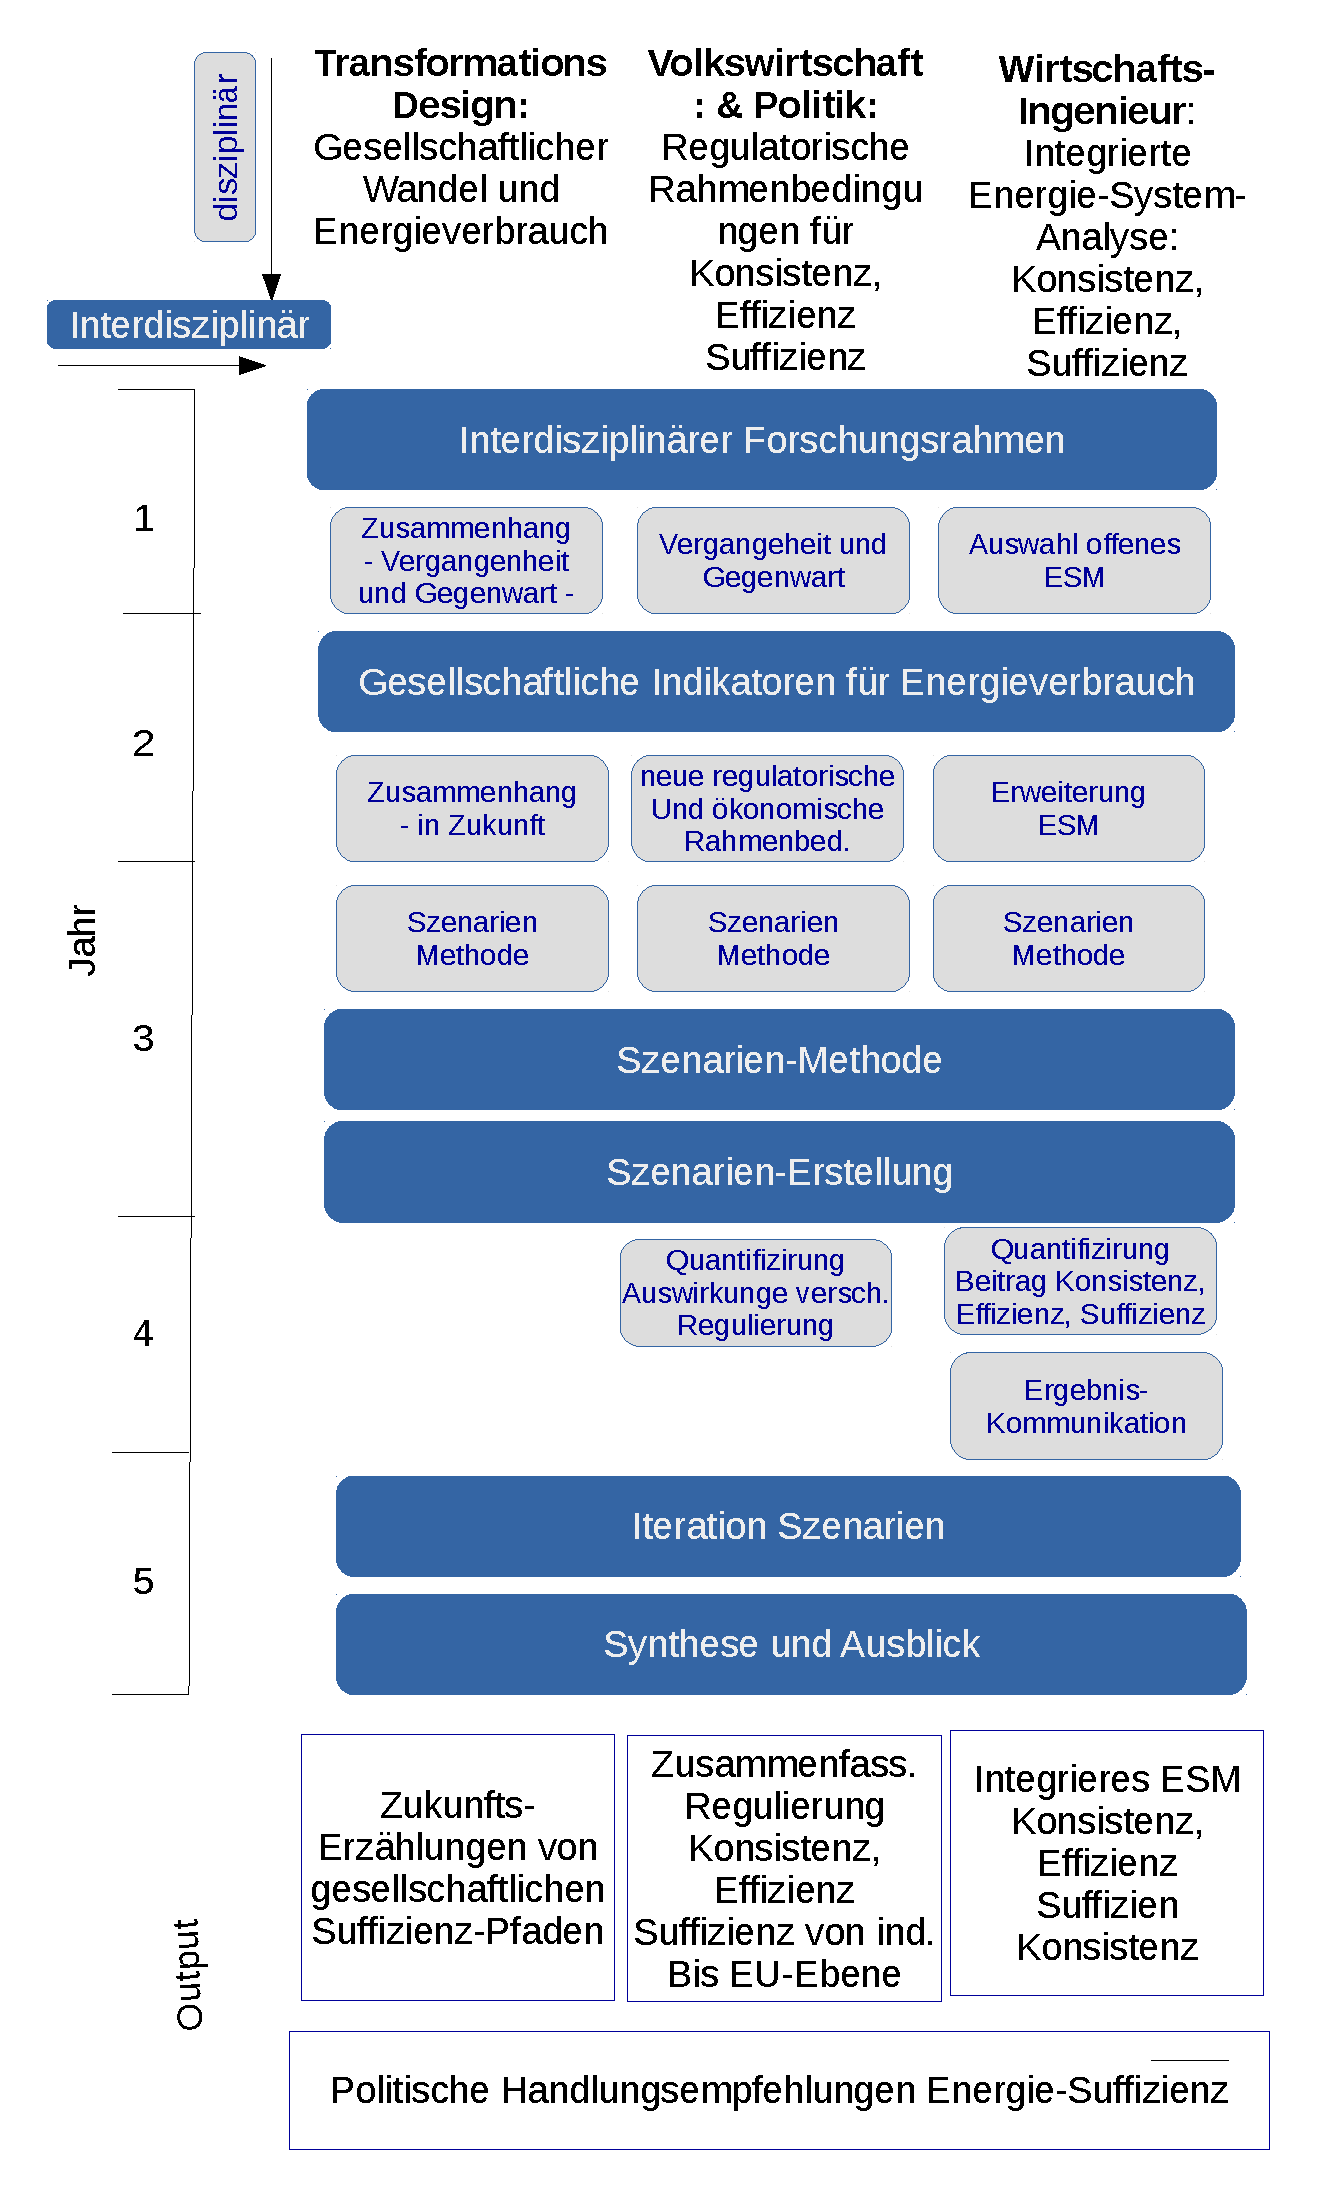
\includegraphics[width=0.8\textwidth]{figures/Forschungsarbeit.pdf}
    \caption{Forschungsprogramm: Disziplinäre Forschungsarbeit (vertikal) und  interdisziplinäre (horizontal) Arbeitspakete im Verlauf der fünf Jahre sowie geplanter disziplinärer und interdisziplinärer Output}
    \label{fig:forschungsprogramm}
\end{figure}

Abbildung \ref{fig:forschungsprogramm} gibt einen Überblick wie die disziplinären Forschungsfelder (vertikal dargestellt) im Verlauf der fünf Jahre über die interdisziplinären Arbeitspakete (horizontal dargestellt) ineinander greifen. Im Folgenden wird jedes Forschungsfeld mit Meilensteinen sowie die interdisziplinären Arbeitspakete kurz erläutert.

\subsection*{Forschungsfeld sozial-ökologische Transformationsforschung: Gesellschaftlicher Wandel und Energieverbrauch}
\textit{NEC: Bitte ergänzen}
Vergangene umfassende gesellschaftliche Transformationen sind immer mit einer Veränderung der energetischen Basis von Gesellschaften einher gegangen, dies ist in der sozial-ökologischen Forschung verschiedentlich herausgearbeitet worden. Die am Norbert Elias Center angesiedelten Promotionen folgen dieser Erkenntnis insofern, als in einer Arbeit in historischer Perspektive Zusammenhänge zwischen Energieverbrauch und sozialem Wandel insbesondere seit den 1950er Jahren herausgearbeitet werden. Die zweite Arbeit ist dem Blick in die Zukunft gewidmet. wie gesellschaftliche Veränderungen und Trends künftig mit Energieverfügbarkeit und -nachfrage interagieren werden. Ausgehend von bestehenden Szenarien und Erzählungen aus der sozial-ökologischen Forschung (WBCSD 1997; WBGU 2011; Öko-Institut 2017) bzw. der Sozialforschung (Wallerstein et al. 2014) werden unter anderem folgende Fragen gestellt: Was bedeuten die gegenwärtigen Trends für mögliche Zukünfte? Welchen Auswirkungen gesellschaftlicher Entwicklungen etwa im Bereich der Demographie, der Migration oder der Digitalisierung auf Wohnflächennutzung (und damit Wärmebedarf), Mobilität oder Strom etc. ist zu rechnen? Was sind jeweils zu erwartende Implikationen für Energieverbräuche und welche Potenziale der Energie-Suffizienz beinhalten sie? Neben „klassischen“ Forecasting-Szenarien (Kosow und Gaßner 2008) kann hier möglicherweise auch ein transdisziplinäres Verfahren aus der Zukunftsforschung zum Einsatz kommen: Mittels Backcasting (Robinson 2003; Robinson et al. 2011) lässt sich ausgehend von einer normativen Vision für eine wünschbare Zukunft – etwa einer lebenswerten Gesellschaft, die ohne (auch externalisierte) Emissionen im Energiebereich auskommt („Null Emissionen bis 2050“) – methodisch kontrolliert abschätzen, welche notwendigen Schritte auf dem Weg in diese wünschenswerte Zukunft gegangen sein und welche Verhaltens- und gesellschaftlichen Veränderungen bis zum Zieljahr vollzogen worden sein müssten. 
Aus beiden zeitlichen Perspektiven – der historischen Rekonstruktion wie dem Blick auf mögliche Zukünfte – werden sich Möglichkeiten und Grenzen (etwa aufgrund von Pfadab-hängigkeiten, nichtintendierten Nebenfolgen, Rebound etc.) für einen suffizienten Umgang mit Energie bzw. eine absolute Reduktion des Energieverbrauchs ableiten lassen  

\textbf{Meilensteine}
T1: Zusammenhang gesellschaftlicher Wandel und Energieverbrauch - Vergangenheit und Gegenwart\\ Historische Rekonstruktion
T2: Zusammenhang gesellschaftlicher Wandel und Energieverbrauch - Zukunft Szenarien-Methode\\
...\\
T Output: Zukunftserzählungen von gesellschaftlichen Suffizienz-Pfaden

\subsection*{Forschungsfeld Politikwissenschaft: Suffizienz-Politiken und Rahmenbedingungen}
\textit{Wuppertal: Bitte umformulieren/ergänzen}
\textbf{Meilensteine}
Ö1: Regulatorische und politische Rahmenbedingungen für Konsistenz, Effizienz und Suffizienz - Vergangenheit und Gegenwart\\
Ö2: Regulatorische und politische Rahmenbedingungen für Konsistenz, Effizienz und Suffizienz - Zukunft\\
Ö3: Szenarien-Methode\\
Ö4: Quantifizierung der Auswirkungen (Emissionsreduktion, Kosten) verschiedener regulatorischer Maßnahmen zu Konsistenz, Effizienz und Suffizienz\\
Ö5: \\
Ö Output: Zusammenfassung Konsistenz, Effizienz und Suffizienz Maßnahmen auf individueller, kommunaler, nationaler und EU-Ebene

\subsection*{Forschungsfeld Systemanalyse: Integrierte Energie-System-Modellierung: Beitrag von Konsistenz, Effizienz und Suffizienz zur Energiewende}

\textbf{Meilensteine}
S1: Auswahl eines offenen Energiesystem-Modells (erweiterbar, anpassbar, open source, gewisser Nutzerkreis)\\
S2: Erweiterung ESM um die ermittelten Nachfrage-Parameter\\
S3: Szenarien-Methode\\
S4: Modellierung: Quantifizierung des Beitrags von Konsistenz, Effizienz und Suffizienz zu einem Energiesystem mit geringem Anteil fossiler Brennstoffen\\
S5: Ergebnis-Kommunikation\\
S Output: Integriertes ESM für Konsistenz, Effizienz, Suffizienz wird unter einer offenen Lizenz Wissenschaft und Gesellschaft zur Verfügung gestellt

\subsection*{AP1: Interdisziplinärer Forschungsrahmen}
Zu Beginn der fünf Jahre wird von allen Wissenschaftler*innen der interdisziplinäre Bezugsrahmen für Forschung zu Energie-Suffizienz aus Sicht der Energiesystemanalyse, der sozial-ökologischen Transformationsforschung und der Politikwissenschaft entworfen. Neben dem inhaltlichen "sich aufeinander einlassen" wird in diesem Arbeitspaket die Zusammenarbeit auch organisatorisch geplant, wie z.B. Häufigkeit der Treffen.

\subsection*{AP2: Gesellschaftliche Indikatoren für Energieverbrauch}
\textit
Um Suffizienz im Energiesystem-Model abbilden zu können, bedarf es einer Übersetzung von gesellschaftlichen Indikatoren zu quantifizierbarem Energieverbrauch. Dieser soziologisch-technisch-ökonomischen Schnittstelle ist dieses AP gewidmet. Hier gilt es gesellschaftlich relevante Einflussfaktoren auf die Energienachfrage zu ermitteln. Diese bilden die Grundlage für die Auswahl der Indikatoren, die in das Energiesystem-Modell als Input-Parameter aufgenommen werden. Zunächst soll es in diesem AP um die historische Rekonstruktion der sozialen Ursachen für Steigerung des Energieverbrauchs gehen. Anknüpfend an den Befund, dass vergangene umfassende Wandlungsprozesse immer mit einer Veränderung der energetischen Basis von Gesellschaften einhergegangen sind (Sieferle 1982; Diamond 2004; Fischer-Kowalski et al. 2011; Haberl et al. 2011), soll historisch nachgezeichnet werden, wie sich mit der Etablierung des fossilistischen Energieregimes in der Vergangenheit Alltagspraktiken in den Bereichen Wärme, Mobilität, Strom (mit einer noch festzulegenden Schwerpunktsetzung, vgl. AP1) verändert haben, welche Implikationen dies jeweils für den absoluten Energieverbrauch hatte und anhand welcher energieverbrauchenden Praktiken sich dies zeigen ließe. Gesellschaftliche Veränderungen und Trends wie eine zunehmende funktionale Differenzierung, Individualisierung, Beschleunigung (Rosa 2005) etc. werden dahingehend befragt, welche Praktiken, kulturellen Deutungsmuster und mentalen Infrastrukturen (Welzer 2011) (etwa der Steigerungslogik) mit ihnen jeweils einhergingen und welche gesellschaftlichen Einflussfaktoren auf die Energienachfrage sich daraus ergeben haben. Insbesondere interessieren hier die Entwicklungen seit den fordistisch geprägten und als Zeit der „Großen Beschleunigung“ bezeichneten 1950er Jahren (Pfister et al. 1995; McNeill 2014). Denkbar wäre etwa in Anlehnung an die Indikatoren, die Will Steffen et. al. (2007) zur Darstellung der Intensivierung des gesamten Naturverbrauchs genutzt haben (fokussiert wurde etwa in globaler Perspektive auf Bevölkerungswachstum aber auch auf McDonalds Filialen, Papierverbrauch oder die Zahl motorisierter Fahrzeuge), Indikatoren zu identifizieren, mit denen suffizientes wie nicht-suffizientes Handeln dargestellt werden kann. In enger Abstimmung wird fortlaufend erörtert, wie sich aus den Wissensbeständen über das historische Gewordensein des Energieniveaus quantifizierbare Indikatoren für den Energieverbrauch ableiten lassen und auf welche Weise diese Eingang in ein umfassendes Energiesystem-Modell finden können. Diese „Übersetzung“ qualitativer in quantitative Einschätzungen wird interdisziplinär erarbeitet.
%Das kann zum Beispiel die EnEV sein, die als Effizienz-Maßnahme zu verstehen ist, da sie nicht auf den Wärmebedarf pro Person sondern auf den Wärmebedarf pro Wohnfläche abzielt. 

\subsection*{AP3: Szenarien-Methode}
In diesem methodischen Arbeitspaket ein Verfahren für die Erstellung von konsistenten, multiperspektivischen Energieszenarien entwickelt. Hierfür ermittelt jedes der drei Forschungsfelder einen Vorschlag für eine Szenario-Methoden, die geeignet ist, Energie-Szenarien im Zusammenhang mit gesellschaftlichen Entwicklungen zu erstellen (siehe Abbildung \ref{fig:szenarien}). Ein Auswahlkriterium soll hierbei die Eignung für die Beteiligung von Praxispartnern in der Szenarienerstellung sein. Im Anschluss an die disziplinäre Vorarbeit geht es dann darum die unterschiedlichen disziplinären Szenario-Ansätze gegenseitig zu verstehen. Darauf aufbauend wird dann in interdisziplinärer Kooperation geprüft, welche Methode geeignet ist um sozio-technische Transformationsszenarien im Hinblick auf Energie-Suffizienz zu erstellen. Ob bestehende disziplinäre Methoden kombiniert und erweitert werden oder bereits bestehende Ansätze wie Kontext-Szenarien genutzt werden, ist Teil des Arbeitspaketes. Eine der Herausforderungen wird die Übersetzung der qualitativen Szenarien in quantitativen Modell-Input sein. Hierbei wird auf die Ergebnisse aus AP2 zurückgegriffen. Ein vielversprechender Ansatz, der in jedem Fall auf seine Eignung geprüft werden sollte, ist die Cross-Impact-Balance-Analysis \cite{WEIMERJEHLE2016}.

\subsection*{AP4:Szenarien-Erstellung}
Im Anschluss an die Auswahl der Methode kommt diese nun zur Anwendung. In der inter- und transdisziplinären Arbeitsphase werden Energiesystem-Szenarien einmal mit Fokus auf Deutschland und einmal mit Fokus auf die Kommune Flensburg erstellt. Im Rahmen von Workshops und Befragungen werden Praxispartner in die Erstellung der sozio-technischen Szenarien einbezogen. Aus den Szenarien werden die Annahmen abgeleitet die Energiesystem-Analyse einfließen. Ein wichtiger Aspekt ist hierbei, dass implizite Annahmen über gesellschaftliche Entwicklungen, die in jedem Energie-Szenario enthalten sind, klar formuliert und bewusst getroffen werden.

\subsection*{AP5:Iteration Szenarien}
Erfahrungsgemäß wird nach der konkreten Übersetzung der Szenarien in quantifizierte Daten und deren Einspeisung ins Energiesystem-Modell deutlich welche Eingangs-Parameter besonders großen Einfluss auf die Ergebnisse haben. Manche Parameter mögen einen größeren Einfluss haben als angenommen, andere haben vielleicht keinerlei Einfluss auf die Konfiguration des Systems und eventuell treten sogar Parameter zu Tage die weitere implizite Annahmen über die gesellschaftliche Entwicklung beinhalten. Deshalb werden die Ergebnisse zuerst interdisziplinär verifiziert und validiert um im Anschluss die Szenarien in mindestens einer Iteration-Schleife anzupassen und zu erweitern.

\subsection*{AP6:Synthese und Ausblick}
Im letzten Teil des Projektes steht die Synthese-Phase der Ergebnis, die als Ergänzung zu disziplinären Publikationen einen Fokus auf die die Publikation von interdisziplinären Methoden, Erfahrung und praktische Verwertbarkeit der Ergebnisse legt. Dies geht Hand in Hand mit einer Ausblicks-Phase, in der Nachwuchs-Forscher*innen sich mit weiteren Qualifizierung- und interdisziplinären Projektmöglichkeiten beschäftigen

\section{Kooperationen, Forschungs- und Praxispartner}
\textit{vorgesehene Kooperationen (Forschungs- und Praxispartner) und Arbeitsteilung, Einbindung der Praxispartner in den transdisziplinären Forschungsansatz}\\

% Allgemein EUF EUM NEC Wuppertal
% Frage: welche Abteilung im Wuppertal Institut?
Die Nachwuchsgruppe ist am interdisziplinären Institut für Umwelt-, Sozial- und Humanwissenschaften der Europa-Universität Flensburg (EUF) und dem Wuppertal Institut für Klima, Umwelt, Energie angesiedelt. Das Forschungsfeld der sozial-ökologischen Transformationsforschung der Nachwuchsgruppe iist am Norbert Elias Center für Transformationsdesign und Forschung verortet während die Abteilung Energie- und Umweltmanagement den Teil der Energie-System-Analyse übernimmt. Beide Abteilungen sind Teil des interdisziplinären Instituts an der EUF und verstärken damit ihre Zusammenarbeit auch innerhalb des Instituts. Am Wuppertal Institut wird das Forschungsfeld Suffizienz-Politk bearbeitet. Die interdisziplinären Arbeitspakete werden in enger Kooperation zwischen der Universität und der außeruniversitären Forschungseinrichtung durchgeführt. In mindestens halbjährlich stattfindenden Treffen aller Mitarbeiter*innen der Forschungsgruppe werden Forschritte diskutiert und Arbeitsschritte geplant, unterstützt von der Mentorin. Diese Gesamttreffen werden flankiert von weiteren bilateralen Arbeitstreffen und intensiven Phasen der interdisziplinären Forschungsarbeit durch mehr-monatige Forschungsaufenthalte in der Partner-Institution durch die Doktoranden. Der genauere Rahmen für die Zusammenarbeit wird im ersten Jahr der Konstituierung der Gruppe gemeinsam festgelegt.

% Leitung geteilt
Zur Verstärkung des interdisziplinären Charakters wird die Forschungsgruppe zu gleichen Teilen von der EUF und dem Wuppertal Institut geleitet (jeweils eine 0,75-Stelle). Dies trägt auch zur engeren Kooperation zwischen Universität und außeruniversitärer Forschungseinrichtung bei.

% allgemein Netzwerke Suffizienz
Weitere Kooperationen außerhalb der Verbundpartner besteht bereits im Suffizienz-Forschungsnetzwerk, ein informeller Zusammenschluss von Forschenden im deutschsprachigen Raum, um den interdisziplinären Austausch zum Thema Suffizienz voranzutreiben und Impulse zur weiteren Untersuchung des Themas zu liefern. Die Nachwuchswissenschaftler*innen werden an den halbjährlich stattfindenden Netzwerk-Treffen teilnehmen.

% EUM Kooperationen
Der Bereich Energiesystemanalyse bringt die bereits bestehende Forschungskooperationen mit der Open Energy Modelling Initiative \cite{}
einbringen. Da hierin so gut wie alle in Deutschland ansässigen Institutionen, die offene Energiesystem-Modellen betreiben, vertreten sind, ist dies besonders hilfreich für die Wahl und Nutzung eines der bestehenden Energiesystem-Modelle. Ob das von der Abteilung EUM in Kooperation mit der Zentrum für Nachhaltige Energiesysteme und dem Reiner Lemoine Institut erarbeitete Energiesystemmodellierungs-Framework 'oemof' in der Nachwuchsgruppe genutzt und erweitert wird, bleibt einer genauen Prüfung und dem Vergleich mit anderen Optionen vorenthalten. 

% NEC Kooperationen?

% Wuppertal Kooperationen?


% Praxispartner
Desweiteren ist eine enge Zusammenarbeit mit den Praxispartnern Stadt Flensburg und Klimapakt Flensburg bei der Szenarienerstellung und -bewertung geplant. Im Rahmen von Workshops bringen Akteure aus Stadt- und Verkehrsplanung, Kommunalverwaltung, Gebäudeverwaltung, Bildung und Klimaschutzmanagement ihr Praxiswissen ein. Auch in der Phase der Bewertung von Modellierungsergebnissen und Anpassung der Szenarien ein nehmen sie eine wichtige Rolle ein. Ein Letter of Intent ist dem Anhang beigefügt.


\section{Betreuungskonzept}
\textit{(inklusive der/des vorgesehenen Mentorin bzw. Mentors und Nachweis deren/dessen Expertise in Bezug auf inter- und transdisziplinäre Forschung}

\textit{Wuppertal: 1-2 Sätze Betreuungskonzept WI und Nachweis Expertise in Bezug auf inter- und transdisziplinäre Forschung der Mentorin.}

Die Gruppenleiterin Frauke Wiese betreut die Promotion in der Energiesystemanalyse, der Gruppenleiter des Wuppertal Instituts im Bereich Suffizien-Politiken, während die disziplinäre Betreuung der beiden Promotionen im Bereich sozial-ökologische Transformationsforschung im Rahmen des Transformationskollegs des Norbert Elias Centers erfolgt (Leitung: Prof. Dr. Harald Welzer, Koordination und Organisation: Dr. Michaela Christ und Dr. Bernd Sommer) und von jeweils einer der Gruppenleiter*innen interdisziplinär unterstützt wird. Bei der anspruchsvollen Betreuungsaufgabe im Spagat zwischen den Disziplinen unterstützen sich die beiden Nachwuchsgruppenleiter*innen gegenseitig und werden dabei von der Mentorin unterstützt. Zweimal im Jahr findet ein Reflexionstreffen der Gruppenleiter*innen und der Mentorin statt mit Fokus auf die Rolle als Leiter/in und den allgemeinen Fortschritt der Forschungsgruppe. 

Ebenso halbjährlich findet ein Treffen aller Mitarbeiter*innen der Nachwuchsforschungsgruppe statt, in der jede*r den Forschritt des Promotionsprojektes vorstellt. So werden nächste Schritte interdisziplinär geprüft und Probleme können frühzeitig erkannt und diskutiert werden. Die Mentorin der Arbeitsgruppe nimmt an diesem Kolloquien teil. Anschließend an den Fortschrittsbericht der einzelnen Forschungsfelder, werden die interdisziplinären Arbeitspakete besprochen. Jedes der interdisziplinären Arbeitspakete wird von einer der beiden Gruppenleiter organisiert mit Unterstützung einer der Doktoranden. Dadurch sammeln die Doktoranden auch im Bereich der interdisziplinären Arbeits- und Projektplanung Erfahrung. Um ihnen außerdem zu ermöglichen, in die lehrende Rolle hineinzuwachsen, ist die Zweitbetreuung von Masterarbeiten durch die Doktoranden geplant. Zusätzliche Weiterqualifizierung der Promovierenden wird durch mindestes einer Teilnahme pro Jahr an Summer Schools und Kursen erreicht. Die Themenfelder der Weiterbildung beinhalten sowohl Methoden-Kompetenz als auch wissenschaftliches Schreiben und transdisziplinäres Arbeiten. Ein mehrmonatiger Forschungsaufenthalt entweder beim Verbundkoordinator oder in einer noch zu definierenden Institution wird angestrebt.

% FEHLT NOCH: Diskussionsrunden führender Personen aus der SOEF-Fachebene verfolgen und beiwohnen

Die akademische Qualifizierung der Nachwuchswissenschaftler*innen wird außerdem dadurch verstärkt, dass von Anfang an eine Kultur des Publizierens gepflegt wird und die Promotionen kumulativ sein werden. Dadurch werden die Doktoranden von Beginn an an peer-reviewte Publikationen herangeführt. Dies kann zuerst in disziplinäre und dann in interdisziplinären Publikationen münden. Da interdisziplinäres Veröffentlichen eine doppelte Herausforderung ist werden die Promovierenden schrittweise herangeführt.

\section{Institutionen, Zukunftsperspektiven und Ergebnisverwertung}
\textit{Darstellung und Motivation der beteiligten Institutionen sowie Zukunftsperspektiven für die jeweiligen Mitglieder der Nachwuchsgruppe (nicht grundfinanzierte außeruniversitäre Forschungsinstitute haben zusätzlich darzustellen, inwieweit den betreffenden Mitgliedern zeitlich befristete Freiräume eingerichtet werden können, sich zeitweise voll auf ihre Qualifikation zu konzentrieren), erwartetes Ergebnis, Anwendungspotenzial und angestrebte Ergebnisverwertung. Der Verwertungsplan muss konkrete Maßnahmen der Öffentlichkeitsarbeit und des Wissenstransfers (auch von Zwischenergebnissen) beinhalten}

% EUF
An der Europa-Universität Flensburg wurde mit der Einrichtung des Interdisziplinären Instituts für Umwelt-, Sozial- und Humanwissenschaften eine zentrale institutionelle Struktur für disziplin-übergreifende Fragestellungen geschaffen. Die Verankerung der sozial-ökologischen Forschung in Form einer eigenständigen Nachwuchsgruppe würde diese mit dem konkreten Forschungsthema Energiesuffizienz mit Leben füllen. Die Zusammenarbeit der wirtschaftsingenieur-lastigen Abteilung Energie- und Umweltmanagement sowie des sozialwissenschaftlich geprägten Norbert Elias Center gilt als große Bereicherung und fügt sich sowohl in die Forschungsarbeit des Interdisziplinären Instituts für Umwelt-, Sozial- und Humanwissenschaften, als auch in das Leitbild der Europa-Universität Flensburg ausgezeichnet ein. Die Stärkung der inter- und transdisziplinären Forschung und insbesondere des Themenschwerpunktes Energiewende und Gesellschaft entspricht der Identität und der zukünftigen Entwicklung der Hochschule.

\textit{NEC: bitte kurze Beschreibung NEC (nur wenige Säzte) - Kurzfassung von Bernds Vorschlag}

\textit{Wuppertal: bitte kurze Beschreibung WI (nur ein kurzer Abschnitt)}

% Zukunftsperspektiven für die jeweiligen Mitglieder
Nach Ablauf des Projektes werden die Nachwuchswissenschaftler*innen mit ihrer inter- und transdisziplinären Erfahrung in einem gesellschaftlich hochaktuellen Thema bestens aufgestellt sein um ihre wissenschaftliche Karriere in diesem Bereich weiterzuführen. An der EUF werden durch eine perspektivische Verstetigung des Forschungsfeldes Gesellschaftliche Transformation und Energiewende Optionen für eine die interdisziplinäre akademische Laufbahn in diesem Bereich geschaffen. In der letzen Phase der Nachwuchsforschungsgruppe wird der Zukunftsplanung und Analyse der Optionen und Folge-Projekte der beteiligten Wissenschaftler*innen Raum gegeben. 

% Wuppertal Institut?

% Welches Ergebnis erwarten wir und wie kann es von Forschung und Zivil-Gesellschaft genutzt werden?
In Abschnitt \ref{sec:ziel} werden die Ziele der Nachwuchsforschungsgruppe aufgeführt. Der erarbeitete Methode zur konsistenten Szenarienerstellung kann von anderen, speziell interdisziplinär arbeitenden Forschern angewendet und weiterentwickelt werden. Auch das Energiesystem-Modell, dessen Programmier-Code und Daten komplett zur Verfügung gestellt wird bildet eine Basis um auf den Erkenntnissen zu Energie-Suffizienz aufzubauen. Dies ist vor allem durch die Offenlegung des gesamten Modellierungszyklunf von Original-Daten über Szenarien bis hin zu Ergebnis-Verifizierung möglich. Die entwickelten Szenarien selbst erweitern die Landkarte  möglichen Energiewende-Pfade durch das Aufzeigen von Suffizienz-Potentialen sowie Maßnahmen. Erarbeitete Handlungsoptionen für Suffizienz-Politik unterstützen Entscheidungsträgern von kommunaler bis EU-Ebene einen Beitrag zur nachhaltigen Transformation zu leisten.

% Öffentlichkeitsarbeit und Wissenstransfer (konkrete Maßnahmen)
Der wissenschaftliche Wissenstransfer wird durch die Teilnahme an Konferenzen und Workshops sowie dem Forschungsnetzwerk Energiewende sichergestellt. 
% konkrete Netzwerkde von NEC oder Wuppertal?
Ein Lernziel der Nachwuchsforschung ist nicht nur die wissenschaftlichem Verschriftlichung aber auch die Kommunikation der Forschungsergebnisse an Nicht-Wissenschaftler. Der Wissenstransfer soll in Form eines Blogs zum Thema Energie-Suffizienz im weiteren Sinne, einer Ringvorlesung sowie der Teilnahme der Wissenschaftler*innen an Formaten wie ``Science Slam'' geschehen. Die Workshops mit den Praxispartnern sind auch Teil der Öffentlichkeitsarbeit und dienen dem gegenseitigen Wissenstransfer von Zivilgesellschaft, Politik und Wissenschaft. Eine gemeinsame Exkursionsreihe 'Suffizienz-Beispiele in der Praxis' in Flensburg in Zusammenarbeit mit den Praxispartnern wäre wünschenswert.

\section{Zeitplanung und Kostenschätzung}
\textit{Gesamtkosten bzw. -ausgaben, Grobkalkulation von Personal-, Sach- und Reisemitteln, gegebenenfalls Berücksichtigung von Eigenbeteiligung sowie Drittmitteln).}

\textit{Basierend auf den geltenden tarifrechtlichen Regelungen und projektbezogen, können in der Regel maximal vier wissenschaftliche Personalstellen (teilbar) je Nachwuchsgruppe beantragt werden (davon maximal zwei Post-Doktorandinnen oder Post-Doktoranden). Bereits durch öffentliche Mittel grundfinanzierte Stellen können grundsätzlich nicht gefördert werden.
In begrenztem Umfang können auch Assistenz- und Hilfskräfte sowie Sachmittel und Mittel zur Einbindung von Praxispartnern beantragt werden.}
% Brauchen wir ein Gantt-Chart?
Die zeitliche Einordnung und Abfolge der Arbeitspakete kann Abbildung \ref{fig:forschungsprogramm} entnommen werden. Die Kalkulation der Personal-, Reise-, Sach- und Weiterbildungsmittel sind Tabelle \ref{tab:kostenkalkulation} zu entnehmen.

Für die gesamten fünf Jahre werden durchgängig vier Stellen beantragt von denen 1,75 Stellen am Wuppertal Institut und 2,25 Stellen an der Europa-Universität Flensburg verortet sind. Letztere setzen sich aus einer 0,75 die Leitungsstelle (TVL14) und drei Doktoranden-Stellen zusammen (halbe Stellen). Am Wuppertal Institut wird ebenso eine 0,75 Leitungsstelle (TVL14), sowie eine halbe Stelle als Doktorandenstelle (TVL13) und eine halbe Stelle für Betreuungs- und Mentorenarbeit (TVL14) eingeplant. Zusätzlich werden wissenschaftliche Hilfskräfte für 20 Stunden pro Woche und Forschungsfeld eingeplant. Auf die Personalmittel wird ein Overhead von 20\% für die EUF und von 90\% für die außeruniversitäre Forschungseinrichtung Wuppertal Institut veranschlagt.
% Wie erklären wir die weiteren 0,5 Stelle

In den Reisemitteln sind die Teilnahme an Konferenzen ab dem zweiten Jahr sowie an vier Workshops pro Person und Jahr enthalten. Außerdem wurde mit halbjährlichen Treffen in abwechselnd Wuppertal und Flensburg mit allen Personen und zusätzlichen drei bilateralen Treffen pro Jahr kalkuliert. In den Sachmitteln sind neben Literatur und Computer für die Modellierung, ab dem zweiten Jahr Gelder für Open Access Veröffentlichungen enthalten. In die Kategorie Weiterbildung fallen Kursgebühren sowie Summer Schools.

Tabelle \ref{tab:kostenkalkulation} fasst die Kosten je Insititution sowie die beantragte Zuwendung entsprechend der Förderquote zusammen.

\begin{table}[h]
\begin{center}
  \caption{Abschätzung der Gesamtkosten je Kostenkategorie für Energie- und Umweltmanagement (EUM) und Norbert Elias Center (NEC) (beide interdisziplinäres Institut der Europa-Universität Flensburg) und Wuppertal Institut}
  
\begin{tabular}[h]{|l | r | r | r | r|}
\hline
&&&&\\
& EUF EUM & EUF NEC & Wuppertal Institut & \textbf{Summe in Euro}\\
\hline
\hline
&&&&\\
 Personalmittel & 641.015 & 505.225 & 1.474.712 & 2.620.952\\
 \hline
 &&&&\\
 Reisemittel & 63.000 & 63.000 & 50.000 & 176.000\\
 \hline
 &&&&\\
 Sachmittel & 26.000 & 26.000 & 30.000 & 82.000\\
 \hline
 &&&&\\
 Weiterbildung & 18.000 & 18.000 & 15.000 & 51.000\\
 \hline
 \hline
 &&&&\\
 \textbf{Summe}& \textbf{748.015} & \textbf{612.225} & \textbf{1.569.712} & \underline{\textbf{2.929.952}}\\
 \hline
 \end{tabular}
 \label{tab:kostenkalkulation}
\end{center}
\end{table}

\begin{table}[h]
\begin{center}
  \caption{Abschätzung von Gesamtkosten und beantragter Förderung je Institution}
\begin{tabular}[h]{|l | r | r | r|}
\hline
&&&\\
Institution & Kosten [Euro] & Förderquote [\%] & \textbf{beantragte Zuwendung}\\
\hline
\hline
 &&&\\
 EUF & 1.360.240 & 100 & 1.360.240\\
 \hline
 &&&\\
 Wuppertal Institut & 1.569.712 & 90 & 1.412.741

\\
 \hline
 \hline
 &&&\\
 \textbf{Gesamt} & & &\underline{\textbf{2.772.981}}\\
 \hline
 \end{tabular}
 \label{tab:kostenkalkulation2}
\end{center}
\end{table}

\clearpage

%\sectionp*{Literatur} \label{sec:lit}
%\bibliographystyle{plainnat}%elsarticle-num}
\bibliographystyle{elsarticle-num}
%\bibliographystyle{apalike}
\bibliography{literature.bib}

\clearpage
\appendix

\section{Anhang}

Literaturlisten, Lebensläufe und gegebenenfalls Interessensbekundungen von Praxispartnern sind im Anhang beizufügen.

\end{document}
